\subsection{Implicit and Explicit Context}
\label{sec:implicit-explicit-context}
Implicit context refers to the latent relationships and dependencies inferred by capturing the surrounding information environment through mechanisms, such as self-attention for transformers, gating for RNNs, and co-occurrence for Word2Vec. More specifically, the self-attention mechanism 
%allows the model to attend 
guides the model by assigning different weights to more relevant parts of the input sequence to capture dependencies between elements.
Explicit context refers to the information that is clearly stated in the content (e.g., text, image) without requiring additional interpretation or inference to understand. It is provided 
%explicitly provided 
alongside the input sequence to enhance its representation and understanding. Knowledge graphs and ontologies can be used to provide this contextual information as external knowledge. We utilize ConceptNet in this study, which provides external knowledge as a structured representation of real-world concepts and their relationships.

\subsection{Knowledge Embedding Models}
\label{sec:knowledge-embedding-models}

Knowledge graph embeddings, also known as knowledge graph representation learning, are techniques used to represent entities and relationships as dense, low-dimensional vectors. These embeddings capture the semantic relationships and similarities between entities and allow for efficient computation and reasoning in knowledge graph-based tasks. In our study we refer to the knowledge graph as $K_g$. Each triple in $K_g$ is represented as $(h,r,t)$ where the entities relation, head and tail are represented as  $h$, $r$ and $t$ respectively.

\textbf{TransE} \cite{bordes2013translating} is a translational energy-based model that represents entities and relations as vectors of the same Euclidean space $R^d$. For a given triple, score function is defined as $f_r(h,t) = -||h+r-t||_{l_1,l_2}$.
% In terms of vector computation it could be represented as or $ h + r \approx t$. 
% TransE performs linear transformation using the following scoring function:

% \begin{equation}
% f = -\lVert h+r-t \rVert_{\frac{1}{2}}
% \end{equation}
\textbf{RotateE} \cite{sun2019rotate} is a translational based model that represents entities and relations in complex vector space $C^d$ and defines each relation as an element-wise rotation from the head entity to the tail entity. The score function is formulated as $f_r(h,t) = - ||h\odot r - t||$, where $\odot$ is the Hadamard (or element-wise) product. 

\textbf{DistMult} \cite{yang2014embedding} DistMult is a semantic-matching model, where the score of a triple can be computed as the bilinear product which is represented as $f_r(h,t) = h\times r \times t$ where $e_h,e_t \in R^d$ and $r \in R^{d \times d}$. Here, restricting $R$ to a diagonal matrix, the score is computed as $f_r(h,t) = h\times diag(r) \times t$.
% In DistMult, every relation $r$ is represented by a diagonal matrix $M_{r}  \in {R}^{{d} \times {d}}$ and a triple is scored as $f(h,r,t) = {e_h}^TM_rE_t$ where $e_h,e_t \in R^d$.
% and a triple is scored as:

% \begin{equation}
% f(h,r,t)= e^{T}_{h} M_{r} e_{t}
% \end{equation}

\subsection{Example data points with captions}
The following examples are from our dataset. Similar to the example in Section \ref{sec:intro} and Table \ref{tab:generated-caption-two-women}, we generated captions with and without knowledge for Figures \ref{fig:muslim-cap} and \ref{fig:ruler} and provided in Table \ref{tab:generated-captions}.  

\begin{figure}[hbt!]
  \centering
  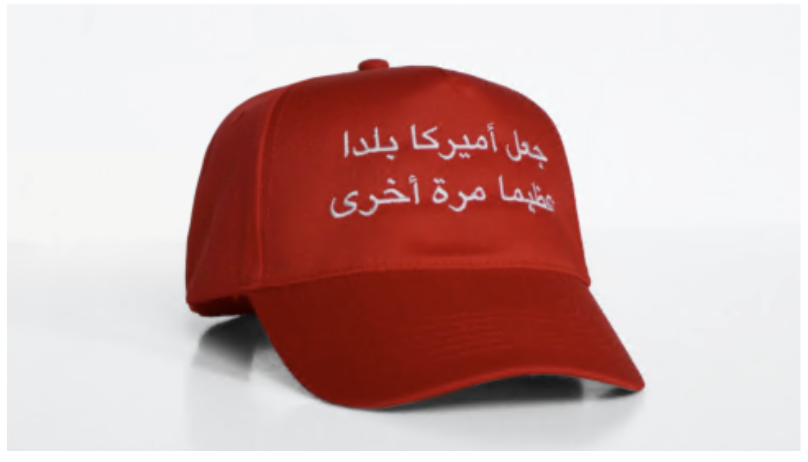
\includegraphics[width=8.5cm]{Figures/muslim_cap.png}
\vspace{-1em}
\caption{\textbf{Actual caption:} "Let's remind everyone that Muslim Americans are a part of our country and that they, too, make America great."}
% \vspace{-1.5em}
\label{fig:muslim-cap}
\end{figure} 

\begin{figure}[hbt!]
  \centering
  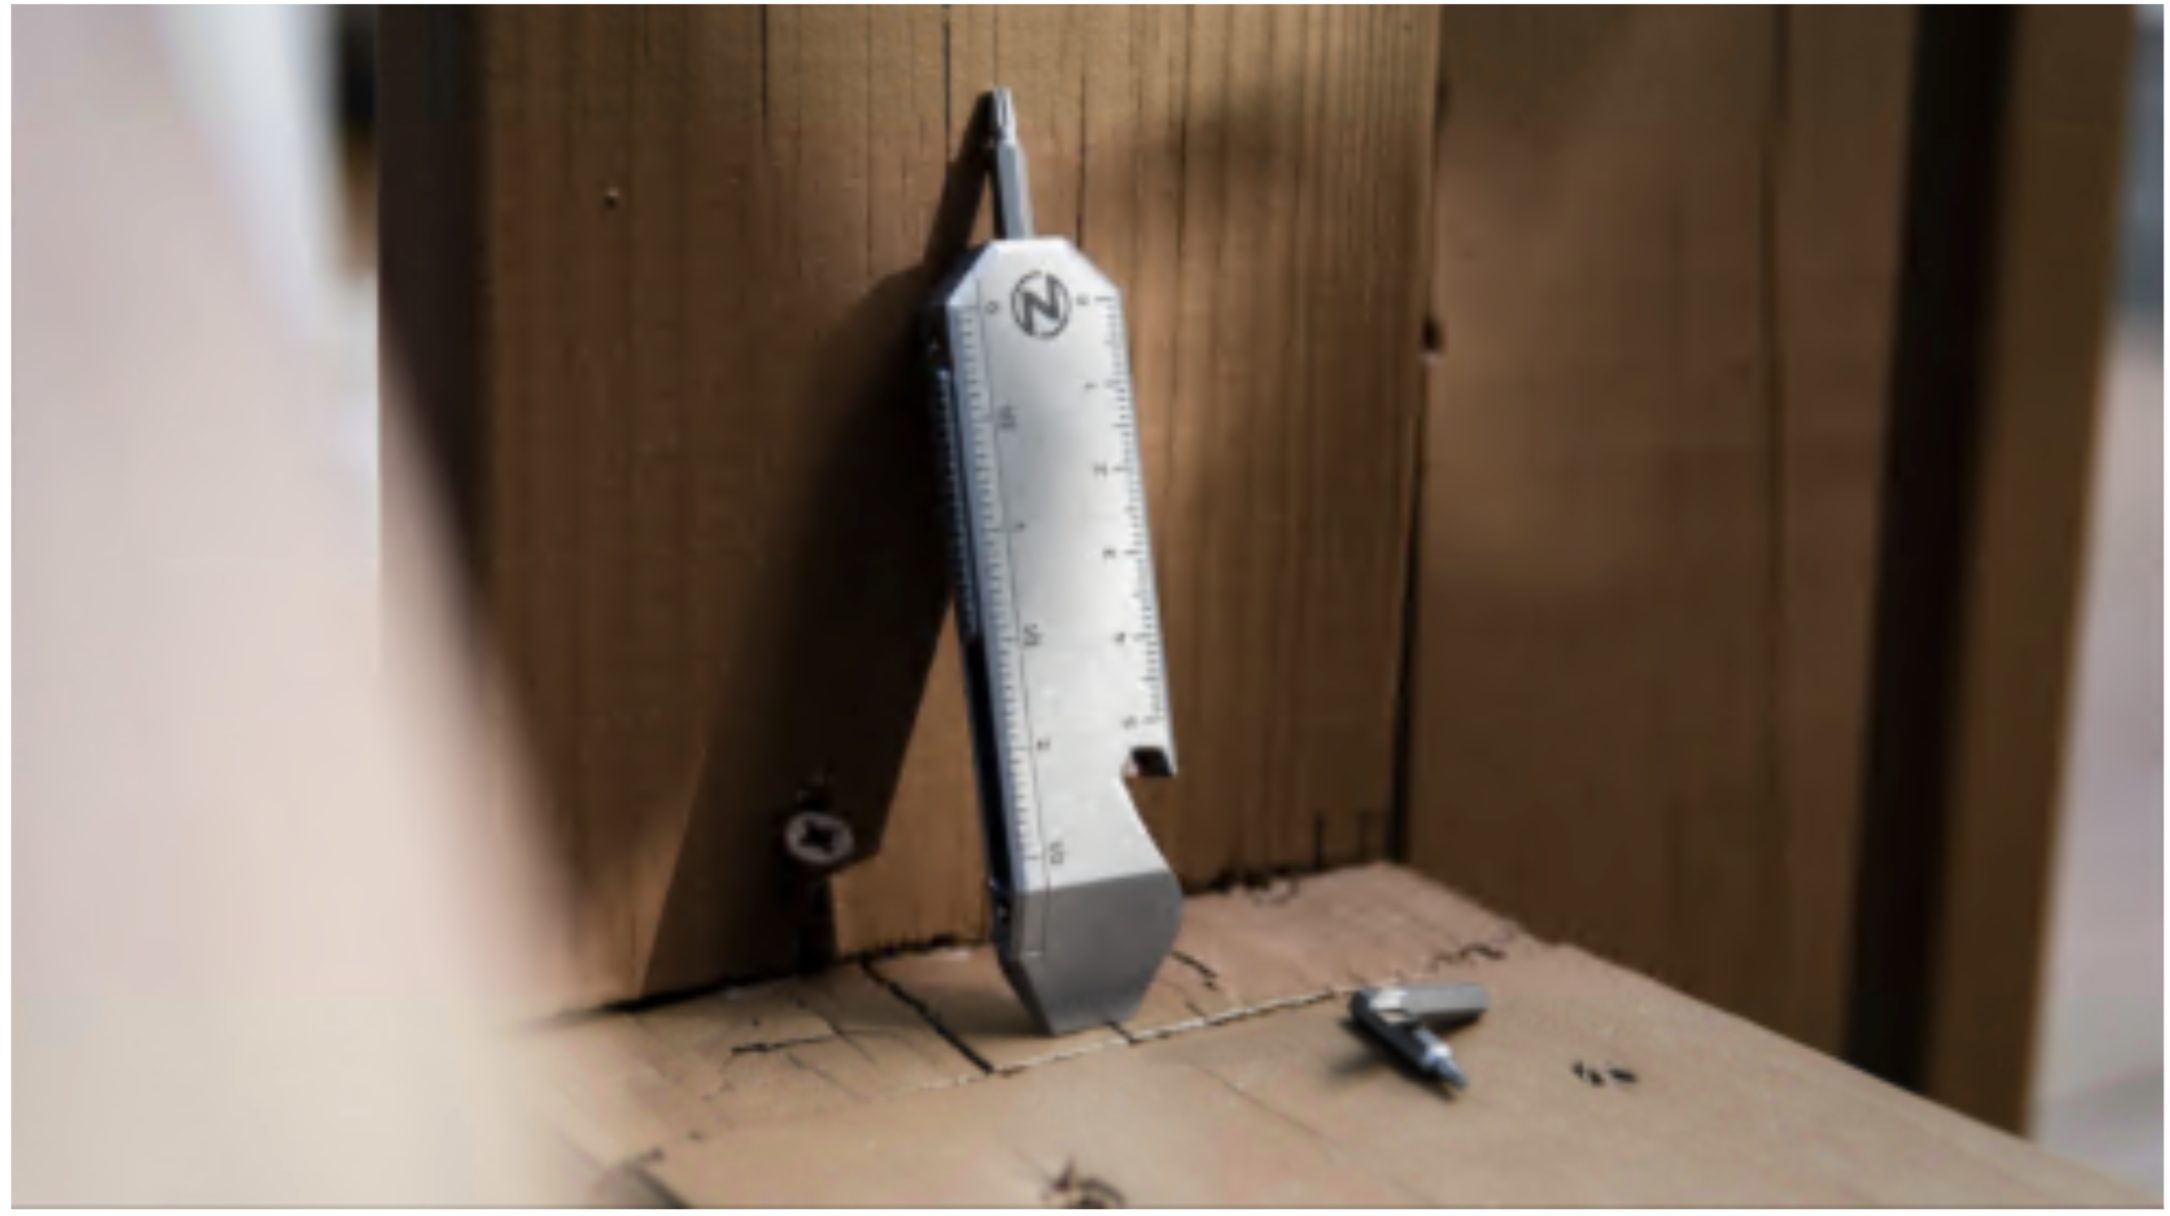
\includegraphics[width=8.5cm]{Figures/ruler.png}
% \vspace{-1em}
\caption{ \textbf{Actual caption:} " A TSA-compliant multi-tool with an innovative internal bit storage compartment"}
\vspace{-1.5em}
\label{fig:ruler}
\end{figure} 

\begin{table*}[!htbp]
  % \setlength\extrarowheight{-2pt}
  \centerline{%
    \begin{tabular}{p{1cm}p{2cm}p{10cm}p{1cm}}
    \toprule[3pt]
   \textbf{Model} & \textbf{Knowledge} & \textbf{Caption} & \textbf{Figure Label} \\
    \toprule[1pt]
    BLIP2 & No& a red baseball cap with arabic writing on it & \ref{fig:muslim-cap} \\
    \toprule[1pt]
    BLIP2 & Yes & muslim Americans are a part of our country and that they, too, make America great
    & \ref{fig:muslim-cap} \\ 
    \toprule[1pt]
    Llava & No & The image features a red cap with white lettering, likely a "Make America Great Again" hat, positioned on a white surface. The hat has Arabic writing on it, suggesting it is meant to convey a message of inclusivity and support for Muslim Americans. The message on the cap reads, "Muslim Americans also make America great." This serves as a reminder that Muslim Americans contribute significantly to the country and are essential in making America great, just like individuals from various backgrounds. & \ref{fig:muslim-cap} \\ 
    \toprule[1pt]
    Llava & Yes & The image features a red cap with white lettering, likely a "Make America Great Again" hat, placed on a white surface. The hat displays Arabic writing, which says, "Muslim Americans also make America great." This message emphasizes the importance of recognizing and appreciating the contributions of Muslim Americans to the nation, reminding people that they, too, play a vital role in making America great. The concept of Americanization refers to the process of adapting to American culture, values, and traditions, and this hat promotes the idea of Muslim Americans actively participating in and enriching the American society. & \ref{fig:muslim-cap} \\ 
    \toprule[3pt]
    BLIP2 & No &  a ruler is sitting on top of a piece of wood
    & \ref{fig:ruler} \\ 
    \toprule[1pt]
    BLIP2 & Yes &  a ruler is sitting on top of a piece of wood
    & \ref{fig:ruler} \\ 
    \toprule[1pt]
    Llava & No &  The image features a silver ruler with an internal bit storage compartment, placed against a brown wooden background. The ruler appears to be a TSA-compliant multi-tool, designed for both measuring and carrying small tools securely while in transit. The ruler's unique storage feature allows it to hold bits or other small objects, making it a practical and convenient tool for various purposes.
    & \ref{fig:ruler} \\ 
    \toprule[1pt]
    Llava & Yes & The image features a silver ruler with an internal bit storage compartment, designed for carrying and organizing small tools or bits securely. \textbf{This TSA-compliant multi-tool is particularly useful for transporting and organizing military equipment or cargo, as it can easily fit into the compartments of aircraft. The innovative internal storage compartment allows for efficient use of space, making it a very handy tool to carry and transport in unmanned transportation devices or the cargo hold of aircraft}
    & \ref{fig:ruler} \\ 
    \bottomrule[3pt]
    \end{tabular}%
  }
\caption{For the image and text pairs (see Figures \ref{fig:muslim-cap} and \ref{fig:ruler}), the captions generated by the models BLIP2 and Llava, when the models were prompted with the Image and Text with and without external Knowledge. The knowledge is extracted from ConceptNet as explained in section \ref{sec:explicit-knowledge} and appended to the prompt input to these models. While the generated captions with knowledge show less hallucinations and more grounding, we leave further investigation of those to the reader as they are not the focus of this study.}
\label{tab:generated-captions}
\end{table*}


\subsection{Extended Exploratory Analysis}[hbt!]
Similar to what we did in the exploratory analysis described in Section \ref{sec:exploratory}, we created clusters for text and image modalities, but in different sizes this time, to show that our observations did not change as shown in Figure \ref{fig:context_congruence_across_data_size}. The clusters get denser and the centroids get closer between them. 


\begin{figure*}
  \centering
  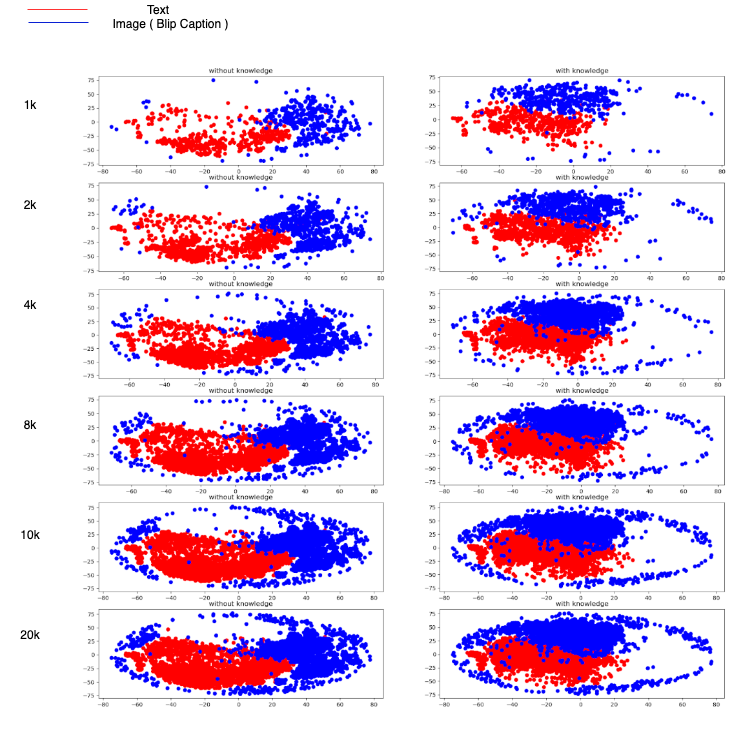
\includegraphics[width=18cm]{Figures/context_congruence_across_data_size.png}
% \vspace{-1em}
\caption{Cluster of the Embeddings of the BLIP Captions and the Marketing Caption Embeddings across varying data sizes. The gap between the image and text clusters reduces in the right plot with the addition of knowledge and can be seen across varying data sizes}
\vspace{-1.5em}
\label{fig:context_congruence_across_data_size}
\end{figure*} 


\subsection{Error Analysis Examples}
As we provided two examples for discussing different outcomes from our experiments including positive and negative, here we provide more examples for the reader to investigate further. The examples include Figures and their explanations
For Figure \ref{fig:error-analysis-woofer-error-analysis}, 
% \textbf{Explanation:} 
The campaign image promotes their 'subwoofer', 'dsp' solution by showing  ‘crowd\_concert’  of fans, their hands raised high in the air. It helps to convey the message  'many\_people\_to\_attend\_concert’.
For Figure \ref{fig:music-album-error-analysis}, 
% \textbf{Explanation:} 
The campaign ad is for a band which wants to promote its music by selling merchandise and by making  its digital copies and their merchandise available for purchase on their website. The band featured in the campaign ad wants to connect with their audience by providing specialized merchandise and releasing their music in digital formats. The noisy entities from the conceptnet ['bridge\_distance\_between\_people', 'bridge', 'bridges', 'bridgeness', 'holding\_up\_bridge']  fail to capture the important events in the pair of image and text.
For Figure \ref{fig:error-analysis-poetry-graffiti}, 
% \textbf{Explanation:} 
The campaign aims to showcase the intersection of 'performance\_poetry' by 'filmmaking'  by capturing these artistic expressions in unconventional locations such as  'graffiti' on  'front\_wall'.The campaign seeks to celebrate both the poet performers and the 'graffitists'.
For Figure \ref{fig:error-analysis-sucess-poet} 
% \textbf{Explanation:} 
Explanation : The campaign image showcases ‘poetry\_book’, ‘books\_of\_poems’, positioned over the ‘wooden\_table’ or the ‘book\_table’.
For Figure \ref{fig:error-analysis-failure-custom-windows}, 
% \textbf{Explanation:} 
The campaign ad is of a company named  “CUSTOMATIC”  which designs custom windows. lot of noisy concepts retrieved such as ‘word\_picture’ which get infused, may confuse the model.


% \vspace{-1.5em}
% \label{fig:custom-windows-error-analysis}
% \end{figure} 

\begin{figure}[hbt!]
  \centering
  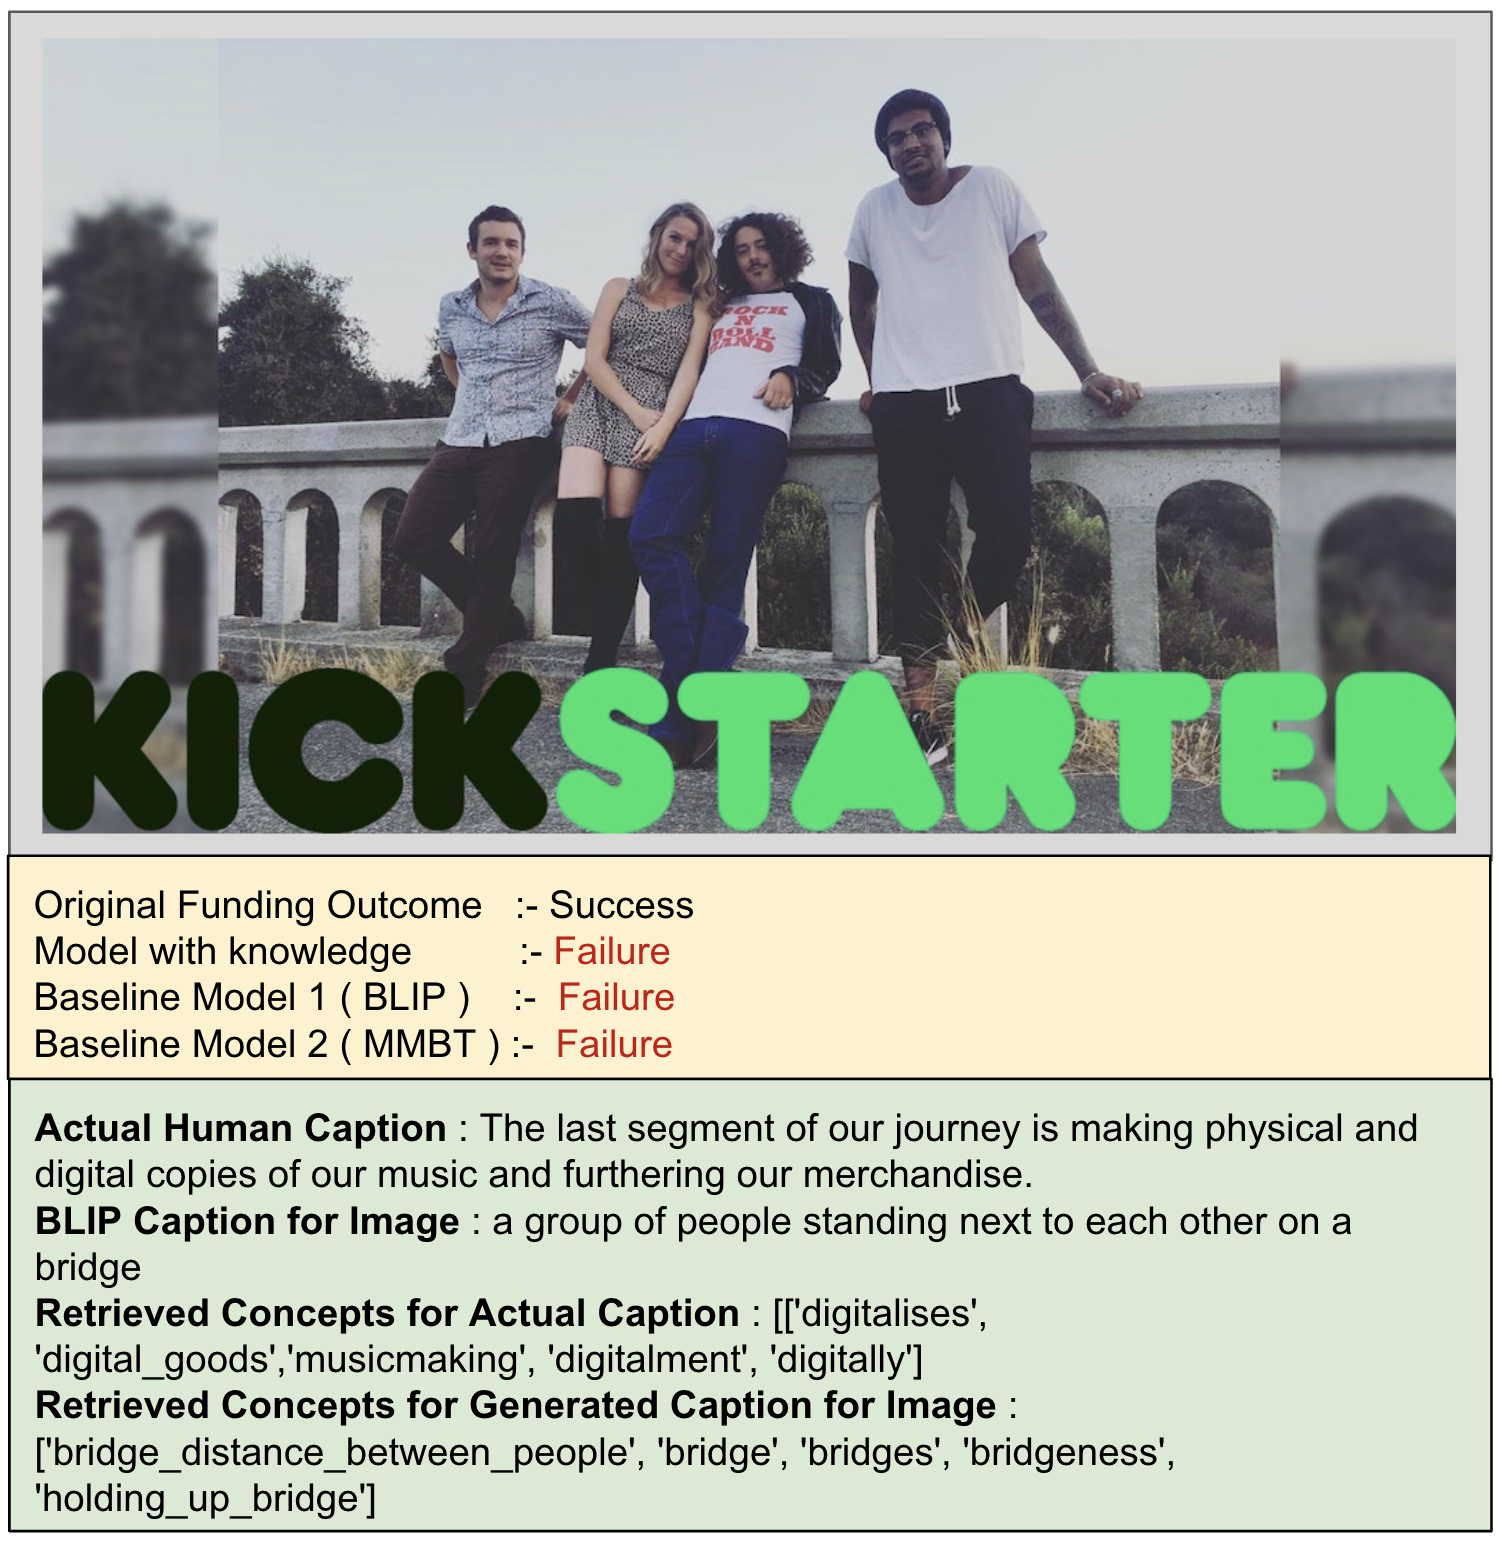
\includegraphics[width=8.5cm]{Figures/erroranalysis/error-analysis-music-band.png}
% \vspace{-1em}
\caption{In the yellow box, the prediction of the model with knowledge, blip model and MMBT, In the green box, actual caption, blip caption, retrieved concepts for each modality.}
\vspace{-1.5em}
\label{fig:music-album-error-analysis}
\end{figure} 

\begin{figure}[hbt!]
  \centering
  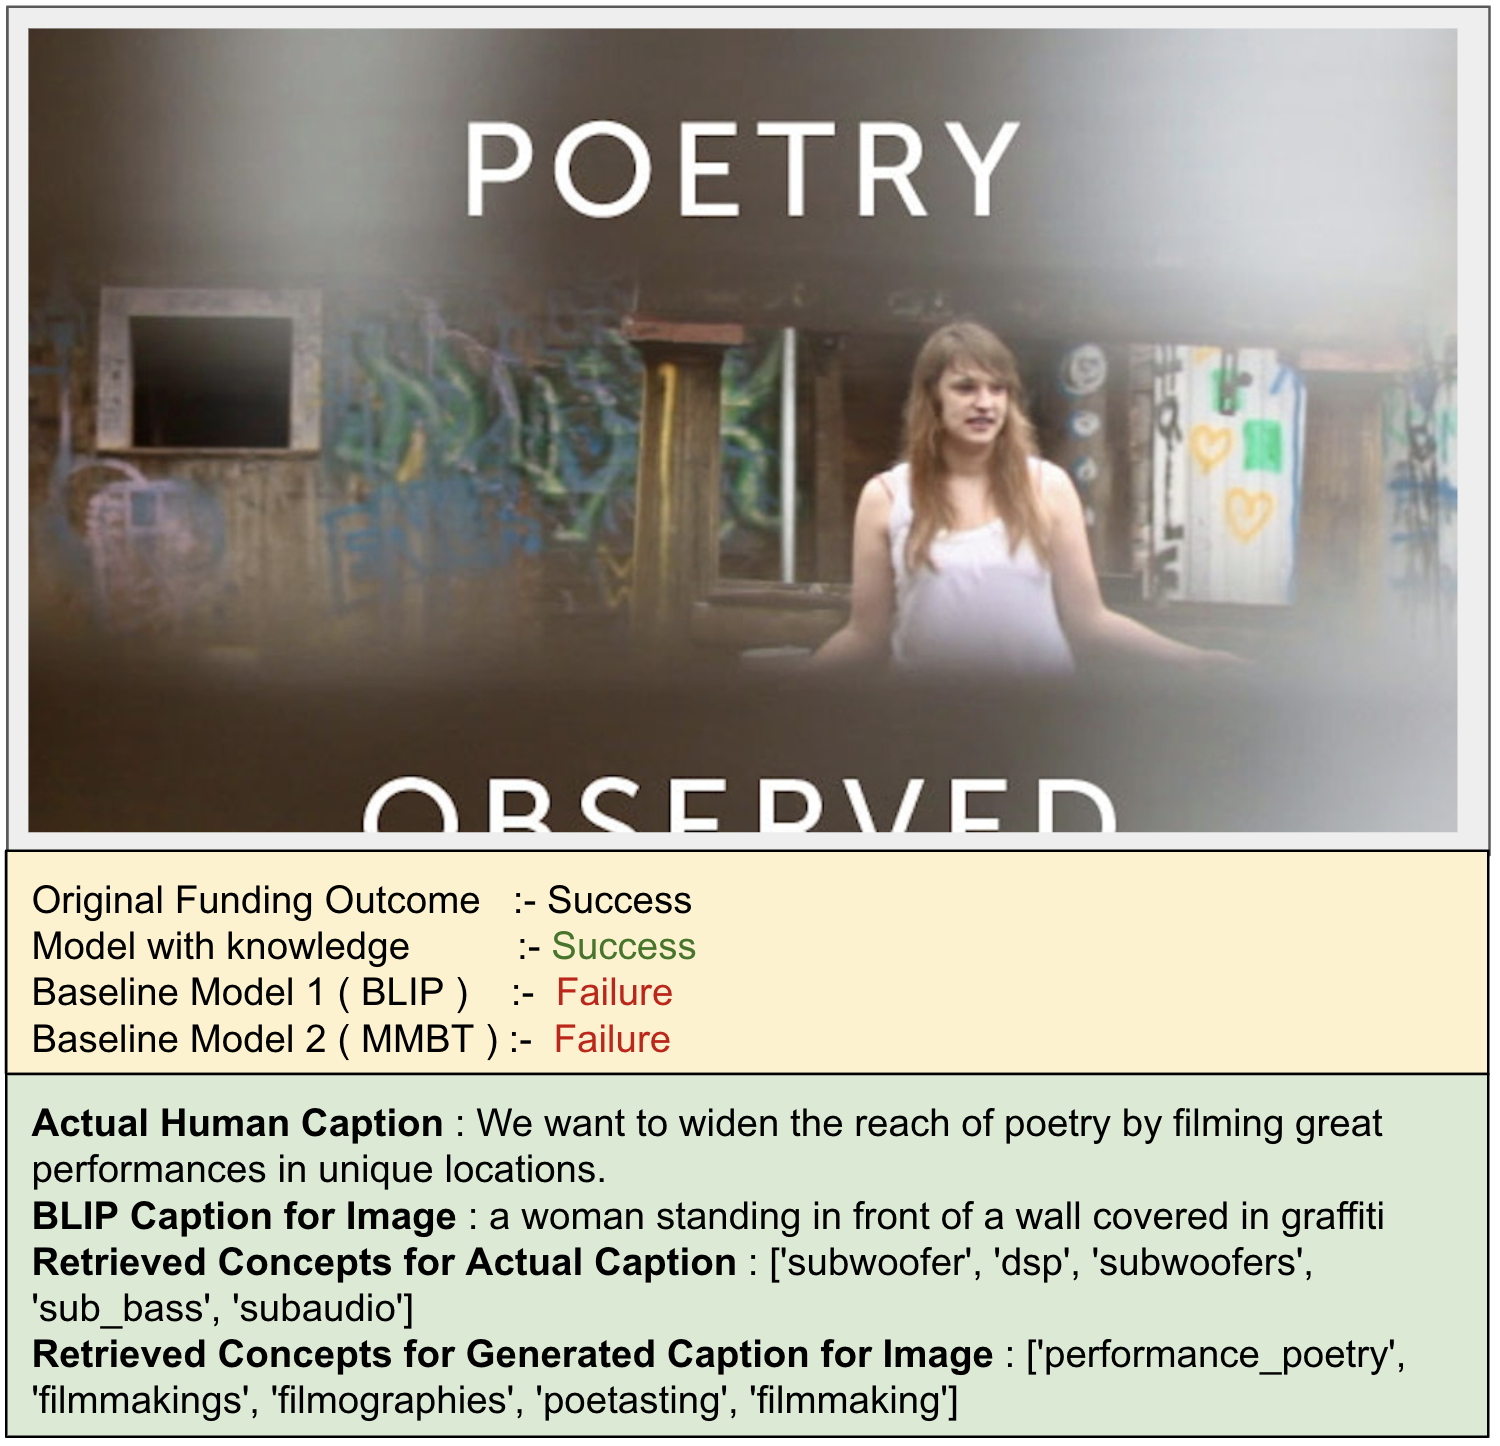
\includegraphics[width=8.5cm]{Figures/erroranalysis/error-analysis-sucess-poet-graffiti.png}
% \vspace{-1em}
\caption{In the yellow box, the prediction of the model with knowledge, blip model and MMBT, In the green box, actual caption, blip caption, retrieved concepts for each modality.\\ 
}
\vspace{-1.5em}
\label{fig:error-analysis-poetry-graffiti}
\end{figure} 


\begin{figure}[hbt!]
  \centering
  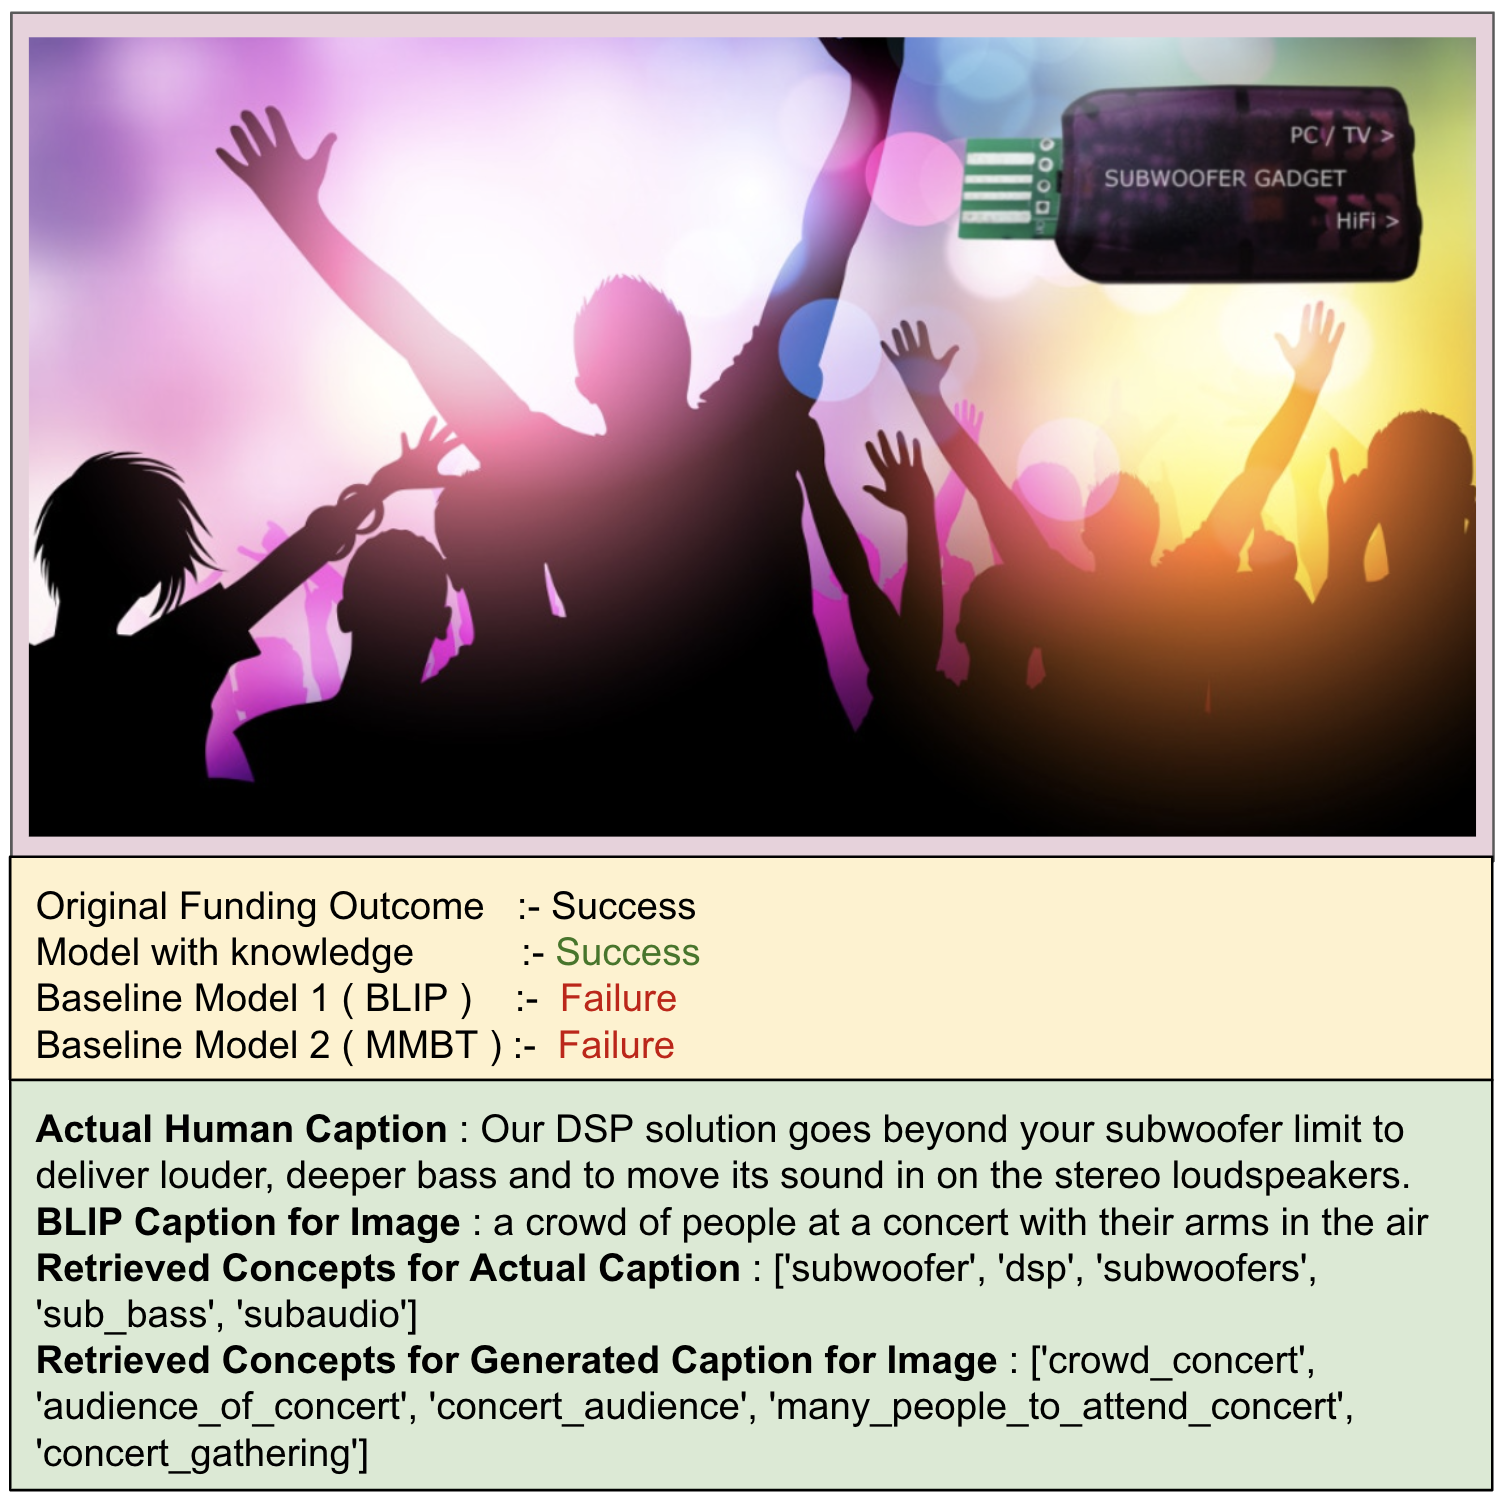
\includegraphics[width=8.5cm]{Figures/erroranalysis/error-analysis-sucess-woofer.png}
% \vspace{-1em}
\caption{In the yellow box, the prediction of the model with knowledge, blip model and MMBT, In the green box, actual caption, blip caption, retrieved concepts for each modality are shown.\\
% \textbf{Explanation:} The campaign image promotes their 'subwoofer', 'dsp' solution by showing  ‘crowd\_concert’  of fans, their hands raised high in the air. It helps to convey the message  'many\_people\_to\_attend\_concert’.
}
\vspace{-1.5em}
\label{fig:error-analysis-woofer-error-analysis}
\end{figure} 

\begin{figure}[hbt!]
  \centering
  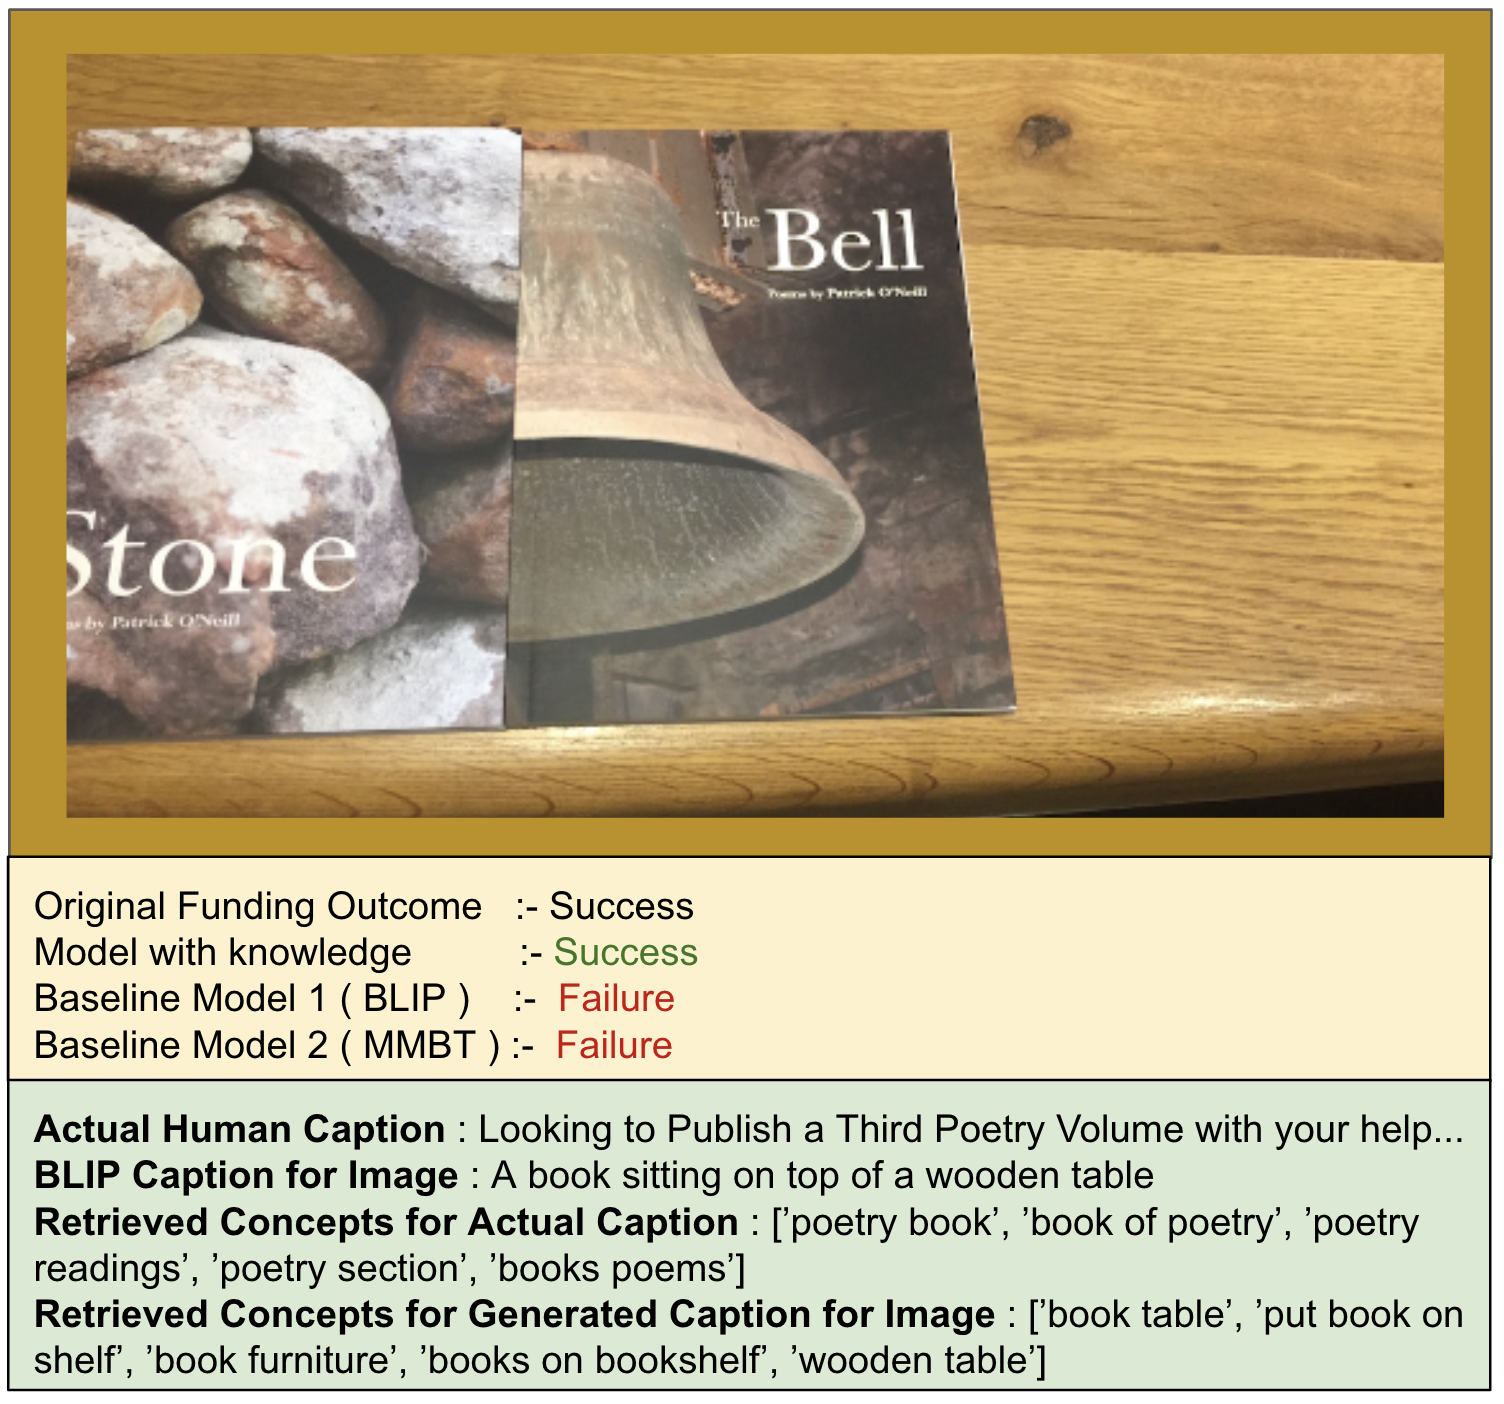
\includegraphics[width=8.5cm]{Figures/erroranalysis/error-analysis-sucess-poet.png}
% \vspace{-1em}
\caption{In the yellow box, the prediction of the model with knowledge, blip model and MMBT, In the green box, actual caption, blip caption, retrieved concepts for each modality.}
\vspace{-1.5em}
\label{fig:error-analysis-sucess-poet}
\end{figure} 

\begin{figure}[hbt!]
  \centering
  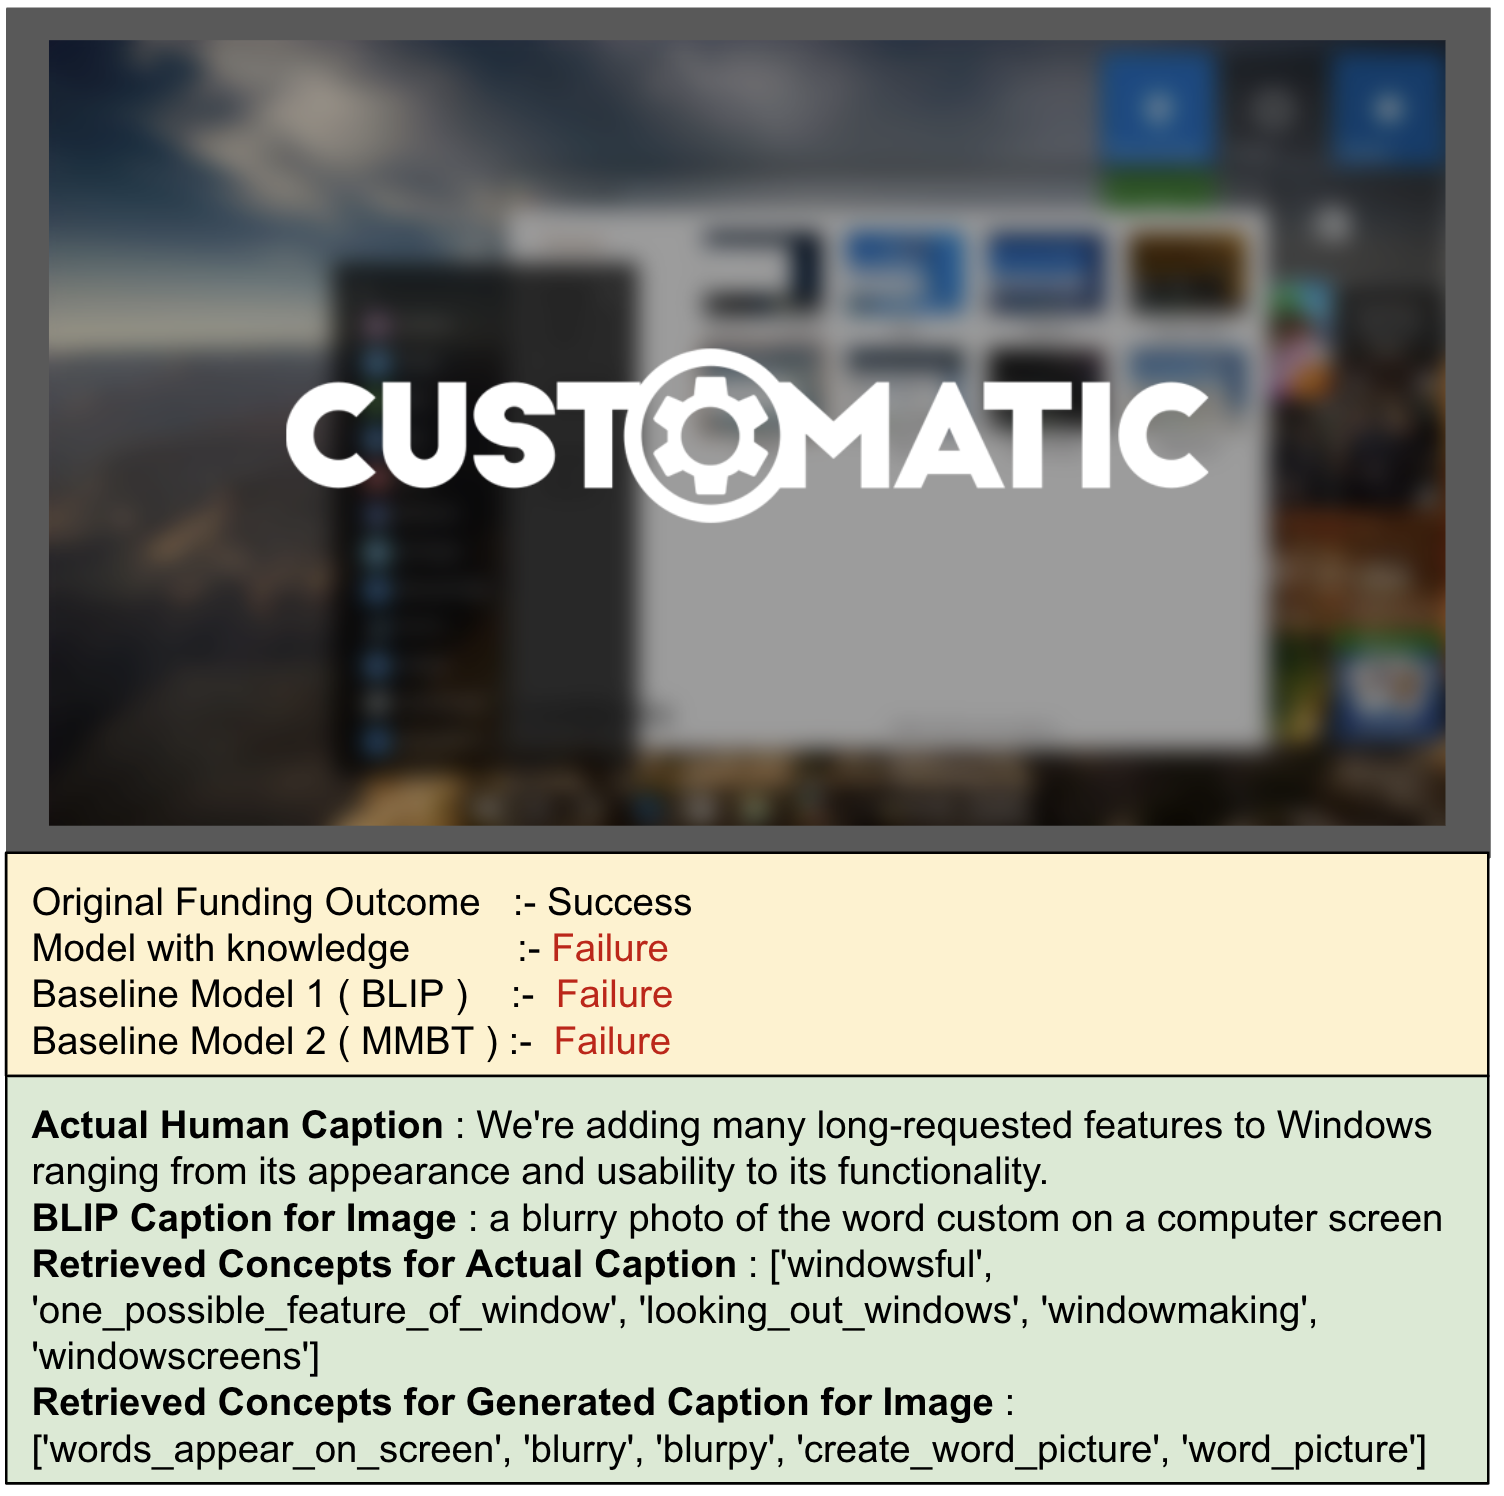
\includegraphics[width=8.5cm]{Figures/erroranalysis/error-analysis-failure-custom-windows.png}
% \vspace{-1em}
\caption{In the yellow box, the prediction of the model with knowledge, blip model and MMBT, In the green box, actual caption, blip caption, retrieved concepts for each modality. \\ 
}
\vspace{-1.5em}
\label{fig:error-analysis-failure-custom-windows}
\end{figure}